\documentclass{MScthesisITEM}

% this package is just to generate text for demo-purposes
\usepackage{blindtext}

\long\def\/*#1*/{}
\usepackage{fancyvrb}
\usepackage[justification=centering]{caption}

\title{High-Level Synthesis for hardware \\architectural exploration} % The title of your assignement; NB use \newlinetitle to start a newline
\author{Jørgen Holmefjord} % Your firstname and lastname
\professor{Kjetil Svarstad, IET} % Affiliation = ITEM for instance
\supervisor{Isael Diaz, Nordic Semiconductor}

%% Uncomment the following in case you want subfigures; note that there will be a warning for the caption package
% \let\subcaption\undefined
% \let\subfloat\undefined
% \usepackage[bf]{caption}
% \usepackage{subcaption}

\DeclareGraphicsExtensions{.pdf,.jpg}
\graphicspath{{./figs/}}

\loadglsentries{glossary}
%\glsaddall[]
%\makeglossaries
\makenoidxglossaries
\begin{document}
\selectlanguage{english}
\pagenumbering{roman}
\pagestyle{plain}

%% Only for the project; comment out the line below for the master's thesis; the front page will be generated automatically by DAIM
\titleITEM

%% Only for the master's thesis; for the project report the description is taken from It's Learning and added by the department
% \selectlanguage{english} % Change to 'norsk' if you are writing in Norwegian
% \begin{titlingpage}

\noindent
\begin{tabular}{@{}p{4cm}p{8cm}}
\textbf{Title:} 	& \thetitle \\
\textbf{Student:}	& \theauthor \\
\end{tabular}

\vspace{2ex}
\noindent\textbf{Problem description:}
\vspace{1ex}

Architectural exploration is a long and complex process where a number of hardware architectures are built and evaluated based on minimum performance requirements and worst-case operational scenarios. With this method, satisfactory results can be achieved if a diverse number of candidates are produced. However, the number of architectures to be evaluated is limited by time and engineering resourced. In this context, High Level Synthesis (HLS) is a compelling alternative to shorten the development time, and consequently, increasing the number of architectures that can be evaluated during the exploration.
Furthermore, by automating the entire architecture exploration process, the optimization engine can take advantage of the higher level of abstraction and generate far more and diverse architectures than it would be possible by parametrized RTL.

The goal of this project-thesis is to set an initial HLS framework in accordance to Nordic Semiconductor's RTL coding policies. This would ensure minimum overhead when integrating to other existing Nordic modules.

There are currently several implementations of HLS by both industry and academia. For this project, LegUp is chosen as the implementation to be used and adapted to our needs. LegUp is open source and has a level of maturity not yet seen in other academic implementations.

Among the goals of this projects are:
\begin{compactitem}
\item Get intimate knowledge of the LegUp libraries that are needed to translate C-code to RTL.
\item Integrate Nordic's coding style and practices into LegUp Verilog libraries, i.e., interfaces, parameters, naming conventions, power/clock domains, etc.
\item Create scripts to automate simulation, synthesis, and power dissipation extraction
\item Create an architectural exploration proof of concept, where a simple design is coded in C and a number of architectures are generated and evaluated in terms of performance, number of gates, and energy consumption.
\end{compactitem}
\vspace{2ex}

\noindent
\begin{tabular}{@{}p{4cm}l}
\textbf{Responsible professor:} 	& \theprofessor \\
\textbf{Supervisor:}			& \thesupervisor \\
\end{tabular}

\end{titlingpage}
% \cleardoublepage

%% There must be an abstract in English, even though the main text is in Norwegian
\selectlanguage{english}
%%\pagestyle{empty}
\begin{abstract}
\noindent
Architectural exploration of digital hardware is an important step in a design process, to find the best trade-off between performance, area, and power consumption based on minimum requirements. Architectural exploration is tedious process, involving many steps to get good results. 

\noindent
This thesis presents the high-level synthesis (HLS) tool, LegUp, and evaluates its usefulness in a design process towards implementation in application-specific integrated circuits (ASIC) hardware. High-level synthesis offers the a potential way to reduce the time and effort put into the process of architectural exploration, by creating a framework that automatically generates multiple Register-Transfer Level (RTL) modules based on a set of architectural variations. 

\noindent
During the work with this thesis, multiple problems were encountered which, in its current state, limits the usefulness of LegUp for ASIC hardware development. The problems can be placed in three categories; input/output, bit-width, and overly complex design. Creating input or output signals in LegUp are not an easy task, as limitations in the compilers and HLS tool forces you to use pointers. Pointers are implemented in a way that requires a dedicated memory controller to handle variables, generating extra overhead and creating the need for a dedicated module for reading and writing to or from the memory controller. This feature is well intended for the focus of the developers to targets design for field-programmable gate arrays (FPGA), but makes things overly complicated for ASIC design. LegUp also lacks the ability to create signals of a given bit-width. This is often necessary when designing modules with control buses or connection to external proprietary devices. Over-sized signals means over-sized modules and functional operations in the internal circuits, leading to additional area and power consumption overhead. The above mentioned memory controller, together with other unused modules generated for FPGA support, makes the output from LegUp overly complex for synthesis towards ASIC implementations.

\noindent
A large section of future works is included, which describes some potential solutions and approaches to make LegUp more suitable for our original intentions. LegUp has potential to be used in a framework for architectural exploration, but this requires that the mentioned issues are resolved first. At this stage, 
\end{abstract}
%%\cleardoublepage

%% Only for the master's thesis; if the main text is in English and you can write Norwegian, there must be an abstract in Norwegian as well.
% \selectlanguage{norsk}
% \pagestyle{empty}
\renewcommand{\abstractname}{Sammendrag}
\begin{abstract}

\end{abstract}
% \cleardoublepage

\selectlanguage{english}% Change to 'norsk' if you are writing in Norwegian

%%\renewcommand{\abstractname}{Preface}
\begin{abstract}
This report is a result of the specialization project in the fifth year of the Master of Science program in Electronics, with specialization in Design of Digital Systems, at the Department of Electronics and Telecommunication (IET) at the \gls{ntnu}. 

The work leading to this report was conducted in the autumn of 2015. This specific project with the title "High-Level Synthesis for Hardware Architectural Exploration" was proposed by the company Nordic Semiconductor ASA in Trondheim, during my summer internship with them in the summer of 2015. I found the subject of High-Level Synthesis interesting, due to my specialization courses at \gls{ntnu} being withing digital hardware design and embedded real-time systems design. Throughout the working period with the project, Nordic Semiconductor have provided me with a workplace and computer equipment with access to their design-tools and other useful resources. I am grateful for the equipment and help I have been given, which were necessary to complete this project.

I would like to thank my supervisors Isael Diaz at Nordic Semiconductor and professor Kjetil Svarstad from NTNU, for their guidance, support and feedback through this project.
\end{abstract}
%%\cleardoublepage

% similarly you may add a separate acknowledgments page

\tableofcontents*
\clearpage
%%\cleardoublepage

%% include if relevant
%%\listoffigures
%%\cleardoublepage

%% include if relevant
%%\listoftables
%%\cleardoublepage

%% include if relevant
%%\listofalgorithms
%%\addcontentsline{toc}{chapter}{List of Algorithms}
%%\cleardoublepage

%% include if relevant
%%\printglossary[title=List of Symbols, style=long]
%%\cleardoublepage


%% include if relevant






%\printglossaries%[title=List of Acronyms,type=\acronymtype] % prints just the list of acronyms
%%\printglossaries
%\printglossary[type=\acronymtype]
%%\clearpage
%%\cleardoublepage
\printnoidxglossaries

\pagenumbering{arabic}
\pagestyle{ruled}
%%\chapter{Introduction}
\label{chp:introduction} 
\section{\label{sec:motivation}Motivation}
The requirements for power efficiency in hardware design is rapidly increasing as more and more end-user products runs on battery. Long battery life is important for many applications, and this demand forces hardware designers to work harder to find the best trade-of between power, area, and performance. Hardware exploration is used to find the best architectural model of a design. This process is very time-consuming as it involves many steps, for instance a \gls{dsp} application design process can include the following steps:
\begin{compactenum}
    \item Make Matlab simulations 
    \item Decide:
    \begin{compactitem}
        \item Quantization
        \item Number of steps of internal modules
    \end{compactitem}
    \item Design$\backslash$choose:
    \begin{compactitem}
        \item The hardware architecture
        \item The ratio of the memories
        \item The type of transistors to use
    \end{compactitem}
    \item ...
    \item Code
    \item Simulate
    \item Extract power consumption
\end{compactenum}
\gls{hls} offers a possible way to shorten this design cycle, by taking advantage of the automatic translation of functional description into digital hardware, one can make optimizations to the system and produce multiple architectural options to choose from. For this project the ultimate goal would be to implement a framework that can automate this process by running optimizations over an entire system and create, simulate, and estimate energy consumption from thousands of architectural variations. This way, the design process is simplified into the following flow:
\begin{compactenum}
    \item Describe circuit functionality in \gls{hll}
    \item Run framework
    \item Select best result from reports
    \item Write \gls{hdl}-code
\end{compactenum}
Traditional \gls{hls}-tools has either been commercial, with very limited access to the source code, or academic open-source tools that were not mature enough for usage in a commercial application. LegUp, the tool examined in this project has reached a maturity not before seen in an academic open-source \gls{hls}-tool. Typically, \gls{hls}-tools generate a large amount of overhead due to the increased abstraction level of the functional specification. By incorporating Nordic Semiconductor's interfaces, coding-style, and practices, described in the \gls{ddvc} \cite{nordicddvc}, into the Verilog generating part of the \gls{hls}-tool, the goal is to reduce this overhead as much as possible, preferably to just a few percentages.

\section{Project objectives}
To achieve the ultimate goal of the project within the time-frame of this thesis, might be a bit optimistic and exaggerated. Some intermediate objectives have therefore been defined, to get some insight into the tools and get started on building a framework:
\begin{enumerate}
    \item Investigate how LegUp performs \gls{hls} and how Verilog is generated. Then look into the possibility of changing or replacing this process in order to generate Verilog suitable for synthesis towards an ASIC architecture. This objective will discover if there are potential problems with LegUp that needs to be handled in order for the other objectives to be achieved.
    \item Specify a \gls{hls} framework that can be used for architectural exploration. The framework shall automatically perform \gls{hls}, simulation, synthesis, layout and estimate power consumption of the design for a variety if different architectural variations and generate score-files, showing the area usage, speed, and power consumption for each alternative. This way the designer can choose design based on design-goals and constraints.
    \item Define a reference design and implement this in both C and Verilog for comparison of area and power consumption between a design written directly in Verilog and multiple \gls{hls}-generated Verilog outputs from a variety of different architectural variations and optimization goals. This will include a design-case compliant to Nordic Semiconductor's \gls{ddvc}.
    \item Make a script that automates the process of the above described framework. The script shall take a file-list pointing to a C-project as input together with constraints and optimization goals like speed, area or power consumption, specified by the user. The framework shall return a score-file, reporting area, speed, and power estimates for each of the targeted architectures.
\end{enumerate}

\section{Overview of the thesis}
\Cref{chp:background} describes the theory of how \gls{hls} and synthesis is performed, with weight on the tools used throughout this thesis. It also presents two reference designs and the theory behind these. \Cref{chp:methodology} gives an introduction to the \gls{hls}-tool, LegUp, and specifies a framework and tool-flow that can be implemented as an automated framework for architectural exploration of digital hardware. The implementation of the reference designs are also presented here. \Cref{chp:resdisc} describes shortly what the output from LegUp looks like. Further multiple problems that were encountered while working with LegUp, are presented and discussed. Finally, \cref{chp:conclusion} sums up the findings and concludes this work. A large section of future work is included in this chapter, to specify what must be handled - and to some extent, how to handle it - in order to achieve the ultimate goal described in \cref{sec:motivation}. Some additional tasks that will improve the framework have been included in the future work-section as well.
\chapter{\label{chp:background}Background}
In the early days of digital hardware design, gate design and layout were performed by hand. With the rapid growth in the numbers of transistors per digital chip design, this method quickly became too time-consuming and thus the need for new and more automated design methods rose. \gls{rtl} design using \gls{hdl} has long been the standard in hardware design, but with the increasing demand for low power and small area in large \gls{soc} designs with multiple billion transistors, this methodology is no longer sufficient if hardware manufacturers want to hit the window of opportunity with their state-of-the-art product.

\section{\label{sec:hls}High-Level Synthesis}

\gls{hls} is not a new concept as it were introduced in research papers in the late 1970 and further researched and developed in the 1980 and early 1990s \cite{martin2009high}. The available commercial \gls{hls} tools has however not been providing the necessary performance and benefits over \gls{hdl} development for major hardware development companies to adapt this methodology until recently.
The concept of \gls{hls} is to use higher abstraction level, often a \gls{hll}, to describe the functional specification of the circuit, and then let a tool help transform this specification into hardware, represented as a \gls{rtl} or \gls{hdl}-model, from given target architectural model libraries and design constraints. The typical \gls{hls}-flow is shown in figure \ref{fig:hlsflow} and each of the transition-steps is described in the below subsections. The input libraries contain information on available hardware resources with power, area, and delay models for the target architecture.

\begin{figure}[hbpt]
\centering
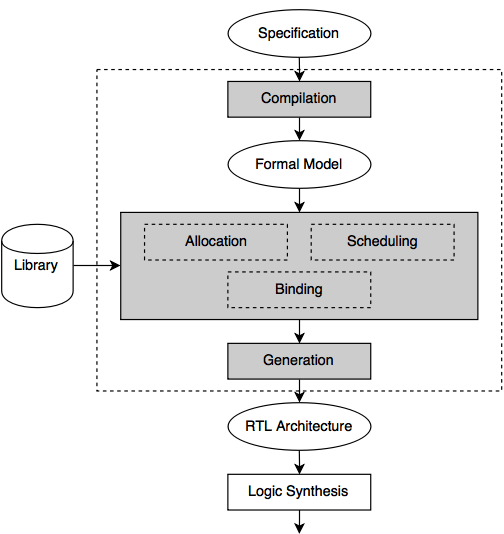
\includegraphics[width=0.6\textwidth]{../figs/HLSFlow.png}
\caption{\label{fig:hlsflow}Information flow in a typical \gls{hls} tool \cite{coussy2009introduction}.}
\end{figure}

\subsubsection{Compilation}

The first step of \gls{hls} is to compile the \gls{hll} into a formal model. This model can vary between different tools, and can be either a specific representation language or a graphic representation of the flow. The formal model is decided by the developers of the \gls{hls} tool. 

\subsubsection{Allocation}

Necessary hardware resources such as functional units, storage and connectivity components needs to be selected from a given \gls{rtl} component library, in order to satisfy the specification and design constraints. Some \gls{hls} tools can also add more resources in scheduling and bind task if found necessary to meet given constraints.

\subsubsection{Scheduling}
Scheduling arranges all operations in an optimized sequence so that variables are read from sources and brought to the input of the correct functional unit for execution and to the destination afterwards. The scheduler takes all dependencies into account when scheduling the operations, in order to get the most efficient result, as some operations can be executed in parallel if no dependencies exist and there is available resources. Operations can be scheduled to finish in one or take multiple clock-cycles and operations can also be chained to eliminate the need for storing the result between operations and to reduce the total number of cycles needed. 
\subsubsection{Binding}
In the binding task, all clock-cycle-crossing variables, operations, and transfers are bound to a free resource in the timeframe when they are scheduled. Non-overlapping or mutually exclusive variables can be bound to the the same storage unit, and operations can be bound to the best optimized functional unit if multiple alternatives are available. Each transfer from component to component, either storage or functional unit, needs to be bound to a connection unit, such as a bus or a multiplexer.
\subsubsection{RTL Generation}
The generated \gls{rtl} usually consists of two parts, a control unit and a data path unit. The control unit is often implemented as a \gls{fsm} that sets control signals to the data path, and controls the current and next-state of the system. The data path contains storage , functional and connection units. Depending on the intensiveness of the binding step, the output \gls{rtl} can be tightly or loosely bound to the available resources. If an operation is not bound to a specific unit, it is up to the following logic synthesis of the \gls{rtl} to bind the operations to available resources. The different types of \gls{rtl} output are illustrated by the following example \textit{a = b * c} executing in state \textit{n}:\\
\begin{minipage}[t][300px]{\textwidth}
\textbf{Without any binding:}%\hfill\vspace{-\baselineskip}
\begin{verbatim}
state (n): a = b * c;
go to state (n + 1);
\end{verbatim}
\textbf{With storage binding:}%\hfill\vspace{-\baselineskip}
\begin{verbatim}
state (n): S(1) = S(2) * S(3);
go to state (n + 1);
\end{verbatim}
\textbf{With functional-unit binding:}%\hfill\vspace{-\baselineskip}
\begin{verbatim}
state (n): a = MUL1 (b, c);
go to state (n + 1);
\end{verbatim}
\textbf{With storage and functional-unit binding:}%\hfill\vspace{-\baselineskip}
\begin{verbatim}
state (n): S(1)=MUL1 (S(2), S(3));
go to state (n + 1);
\end{verbatim}
\textbf{With storage, functional-unit, and connectivity binding:}%\hfill\vspace{-\baselineskip}
\begin{verbatim}
state (n): BUS1 = S(2); BUS2 = S(3);
BUS3 = MUL1 (BUS1, BUS2);
S(1) = BUS3;
go to state (n + 1);
\end{verbatim}
\end{minipage}
A loosely bound \gls{rtl} gives the synthesis the flexibility to optimize the unit binding to updates timing estimates and delays and loads given by the layout and floor-planning.
\section{LegUp}
The \gls{hls} tool used in this project is called LegUp \cite{canis2011legup}. LegUp is an open-source academic tool developed at the University of Toronto, Canada. LegUp's goal is to \textit{"allow researchers to experiment with new \gls{hls} algorithms without building a new infrastructure from scratch"} and their long-term vision is to \textit{"make \gls{fpga} programming easier for software developers"}. LegUp takes \gls{ansi}-C as input and generates synthesizable Verilog \gls{hdl} as output. The developers of LegUp have primarily focused on support for a variety of \gls{fpga} boards from manufacturer Altera, but in the latest version (4.0), beta support for Xilinx devices and possibility to configure the tool to generate generic Verilog to target other \gls{fpga} vendors or even \gls{asic} through use of generic dividers, has been introduced. The big advantage of LegUp compared to similar, commercial tools is that it is open-source and therefore can be configured to target different architectures, and the \gls{rtl} and \gls{hdl} generating part of the tool can be modified or replaced to fit the programmers needs.
Since LegUp, in its unmodified form, targets \gls{fpga} devices, it support three different synthesis flows; pure-\gls{sw}, hybrid, and pure-\gls{hw}. The two first synthesis flows will implement a TigerMIPS \cite{tigmips} soft processor, which will run the whole C program in pure-\gls{sw} flow, while the hybrid flow will run one part of the C code on the soft processor and implement hardware accelerators for functions specified in a constraint file. The pure-\gls{hw} flow will synthesise the whole C file into hardware. It is the pure-\gls{hw} flow that will be the focus of this project.

\subsubsection{Producing Verilog Output}
LegUp is made up of two components; a frontend pass and a target backend pass to the \gls{llvm} compiler infrastructure. 
The information flow in LegUp, shown in figure \ref{fig:legupflow}, follows the same principle as the information flow described in section \ref{sec:hls}.
\begin{figure}[hbpt]
\centering
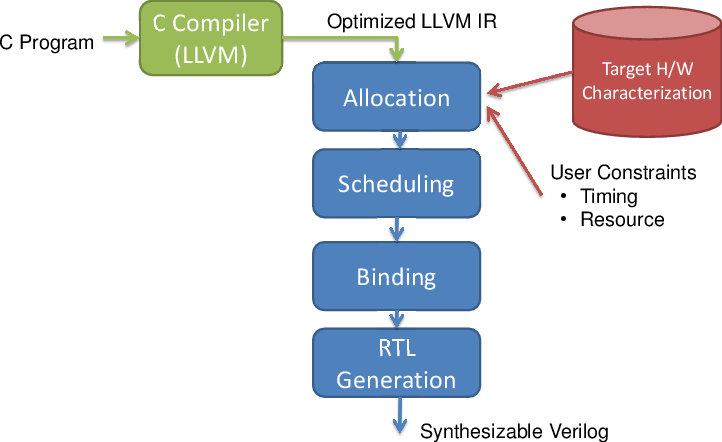
\includegraphics[width=0.6\textwidth]{../figs/LegUpFlow.png}
\caption{\label{fig:legupflow}Information flow in LegUp \cite{legupmaual}.}
\end{figure}
The LegUp \gls{llvm} frontend takes \gls{llvm} \gls{ir} compiled by clang, a C frontend for \gls{llvm}, as input and links in custom written functions like memcpy, memset and memmove, which do not exist in hardware, but that \gls{llvm} assumes exist in the C library. 
The LegUp backend pass performs allocation, scheduling and binding as described in section \ref{sec:hls}. In the next step, \gls{rtl}-module objects that represents the final hardware circuit are generated from each \gls{llvm} instruction. Ultimately, each \gls{rtl}-module is printed to a file using the corresponding Verilog code for the given \gls{hw} module.

\section{\label{sec:LLVM}LLVM}
\gls{llvm} \cite{LLVM:CGO04}, formerly Low-Level Virtual Machine, is a compiler framework that was originally developed as a research infrastructure to investigate dynamic compilation techniques for static and dynamic programming languages, at the University of Illinois in 2000. It is now a open-source project with many contributors from both industry, research groups and individuals, and is used by companies like Apple in their Xcode \gls{ide} \cite{llvmapple} and Sony for their PS4 developer toolchain \cite{llvmsony}. \gls{llvm} support a large number of frontends for programming languages, including Clang \cite{clang} which support C, C++, Obcjective-C and Objective-C++ and is compatible with \gls{gcc}. It also supports a large number of backend target architectures. Figure \ref{fig:llvmcompiler} shows how different source languages can be input to the frontend compiler of LLVM, which translate the source into an \gls{ir}. The \gls{ir} is then optimized using \gls{llvm}s optimizer. At this stage, different source languages can be linked together, and even object files compiled using standard \gls{gcc} can be linked at this stage. The optimized \gls{ir} is then translated into the target architecture by the backend.

\begin{figure}[hbpt]
\centering
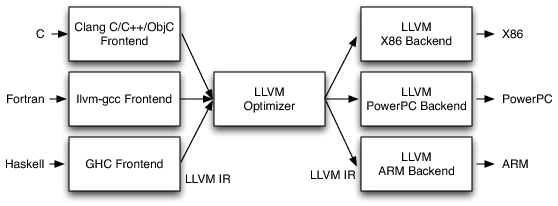
\includegraphics[width=\textwidth]{../figs/LLVMCompiler.png}
\caption{\label{fig:llvmcompiler}LLVMs three-phase compiler structure \cite{llvmarch}.}
\end{figure}

\subsubsection{Intermediate Representation}
\gls{llvm} use a human readable assembly-like, strongly typed RISC instruction set as their \gls{ir}, with support for an infinite number of temporary registers of the form \%0, \%1, etc. \gls{llvm} \gls{ir} can also output a dense bitcode format for serialization.

\section{Alternative hardware design methods}
\gls{hls} is not the only alternative to \gls{hdl}-languages, if you want to design digital hardware at a higher level of abstraction. The following subsections will shortly describe two alternative approaches to digital hardware design. 
\subsection{Chisel}
One interesting approach to designing hardware with a higher level of abstraction, is the Chisel \gls{hcl} \cite{bachrach2012chisel} developed at UC Berkeley. Unlike \gls{hdl} languages like VHDL and Verilog, which were originally designed as simulation languages and later adopted as a basic for synthesis, Chisel was created as a \gls{hcl} and is thus \textit{synthesizable by construction}. This entails that no conversion from C, or other \gls{hll}, into gates is performed, only generation of generic low-level Verilog with no overhead. Chisel is a \gls{dsl} built on Scala \cite{odersky2004overview} with its own syntax, but Scala syntax can also be used to get even greater abstraction in your design. A big advantage using Chisel is its high simulation speed, using C++-based cycle-accurate software simulators.

\subsection{Functional programming}
Functional programming is a relatively different method of hardware design, as it consists only of mathematical functions and immutable data. Two examples of hardware design using functional programming is C$\lambda$aSH \cite{baaij2009clash} and Lava \cite{bjesse1998lava}. Both Lava and C$\lambda$ash are compilers for the functional programming language Haskell \cite{haskellonline}, but while Lava is an embedded \gls{dsl} like Chisel, with its own syntax, C$\lambda$ash use Haskell syntax and semantics, and use a static analysis approach towards synthesis.

\section{\label{sec:powest}Power and area estimation}
In order to compare different use-cases and result generated by LegUp, the area and power-usage will be estimated. Since this is not the main objective of this project, the automated area and power estimation tool-flow created by Joar Talstad in his specialization project \cite{talstad14project} and master thesis \cite{talstad15master} will be adapted for this purpose. This tool-flow use Synopsys Primetime PX for power analysis and estimation.

\section{Information and tool-flow}
LegUp utilizes Makefiles to perform the \gls{hls} flow. The power and area estimation tool-flow described in section \ref{sec:powest} also use Makefiles for its flow. It will thus be suitable to create a single Makefile that controls the information flow from the input of a C file to the output of Verilog files along with scorefiles on the area and power estimates. 

\section{Reference designs}
In order to evaluate the performance and overhead in power and area generated by LegUp, two reference designs is created to compare the produced results from LegUp towards the same design written in native Verilog \gls{hdl}. To evaluate whether the structure of the design impact the overhead on the output, the first design contains a regular structure, where the same operations are performed each clock-cycle. The first reference design was chosen to be a \gls{fir}-filter. The second design contains a state machine, as it is interesting to see if the \gls{fsm} implemented by LegUp generates less overhead if the design itself is a state machine. The choice landed on designing a \gls{sap-1} architecture. Both designs are described in the subsections below.

\subsection{FIR-filter}
\gls{fir}-filter is, together with \gls{iir}-filters, the two categories of linear time-invariant systems, used in digital signal processing application. The impulse response of a \gls{fir}-filter is zero outside some finite time interval.
A general \gls{fir}-filter can be described by the differential equation \cite{proakis2007digital}:
\begin{equation}
    y(n)=\sum\limits_{k=0}^{M-1} b_kx(n-k)
    \label{eq:firfilterdiff}
\end{equation}
or by the system function:
\begin{equation}
    H(z)=\sum\limits_{n=0}^{M-1} b_nz^{-n}
    \label{eq:firfiltersys}
\end{equation}
The impulse response for a \gls{fir}-filter is given by:
\begin{equation}
    h(n)\triangleq
    \begin{cases}
    \begin{tabular}{ll}
      $0,$ & $n < 0$  \\
      $b_n,$ & $0 \leq n \leq M-1$  \\
      $0,$ & $n > M$   
      \end{tabular}
    \end{cases}
    \label{eq:firfilterimp}
\end{equation}
From \cref{eq:firfilterdiff} and \cref{eq:firfilterimp} we get the discrete convolution equation:
\begin{equation}
    y(n)=\sum\limits_{k=-\infty}^{\infty} h(k)x(n-k) \triangleq h(n) \ast x(n)
    \label{eq:firfilterconv}
\end{equation}
\noindent
Figure \ref{fig:firfilter} shows the direct form representation of a N-order \gls{fir}-filter with N+1 taps. 
\begin{figure}[hbpt]
\centering
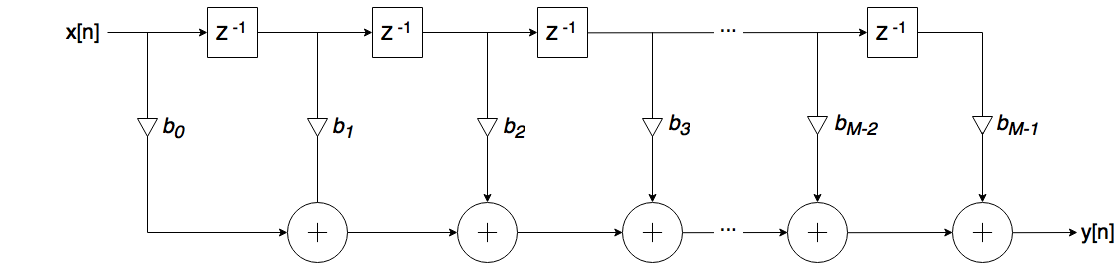
\includegraphics[width=\textwidth]{../figs/FIRFilter.png}
\caption{\label{fig:firfilter}Direct form representation of a N-order \gls{fir}-filter}
\end{figure}
Even though the process of designing a \gls{fir}-filter might not be a trivial task, the implementation of a already designed filter is simple. As seen from \cref{eq:firfilterconv}, the filter can be described by the convolution formula, which implies that the filter can be implemented as convolution of the input function x(n) with the impulse response function h(n).

\subsection{SAP-1 architecture}
The \gls{sap-1} 8-bit architecture were introduced in \cite{malvino1983digital} as a beginners introduction to \gls{cpu}s, which can be implemented using simple hardware components. Figure \ref{fig:sap1arch} shows a block diagram of the \gls{sap-1} architecture. Each block correspond to a hardware component. Signals starting with an asterisk (*) are active low. 
\begin{figure}[hbpt]
\centering
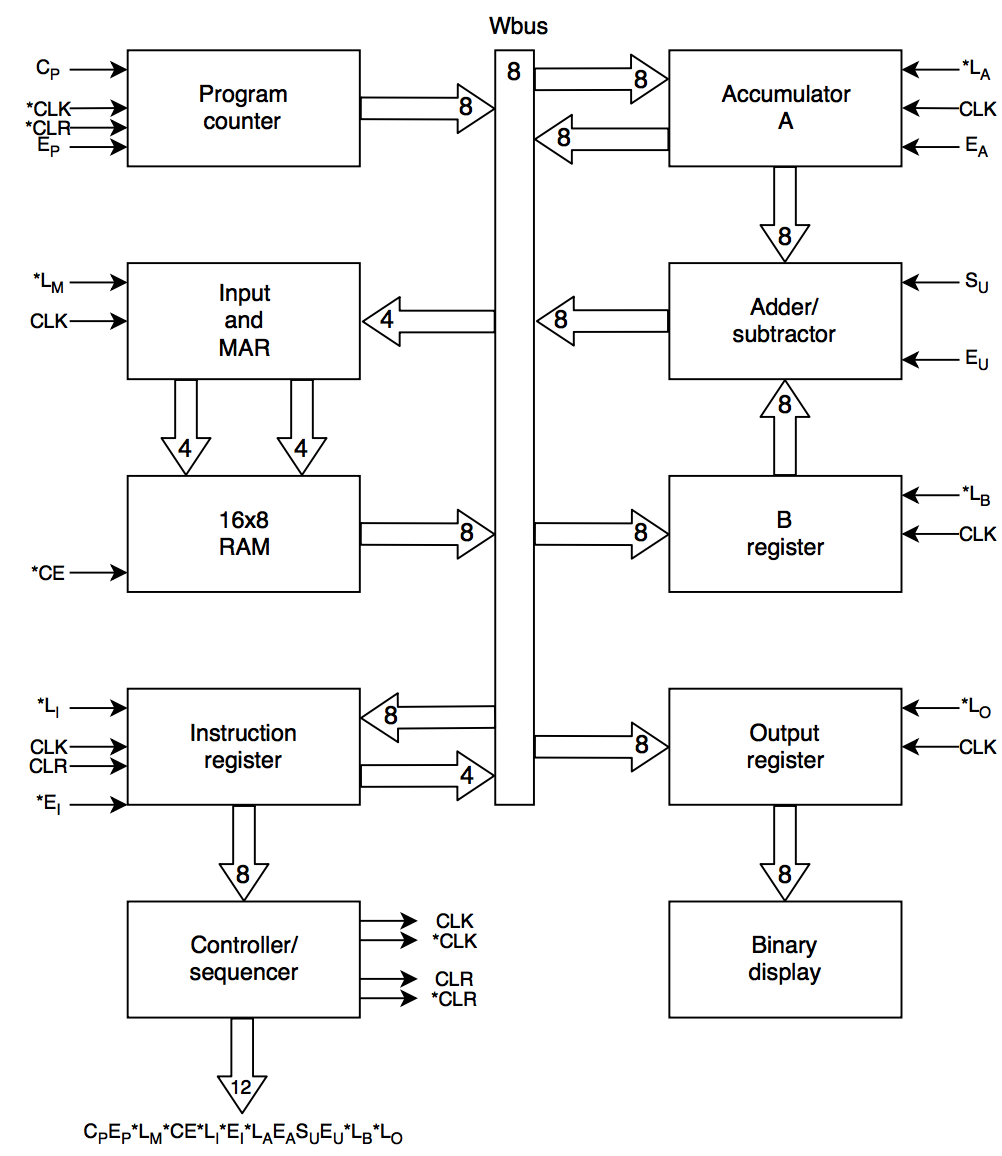
\includegraphics[width=0.6\textwidth]{../figs/SAP1.png}
\caption{\label{fig:sap1arch}Block diagram of \gls{sap-1} architecture}
\end{figure}
The architecture consists of 5 different instructions, listed in table \ref{tab:sap1instr}.

\begin{table}[hbpt]
    \centering
    \caption{\label{tab:sap1instr}Description of instructions in \gls{sap-1} architecture}
    \begin{tabular}{lll}
      \textbf{Instruction} & \textbf{Opcode} & \textbf{Description} \\
      \hline
      LDA & 0000 & Load RAM data into accumulator \\
      \hline
      ADD & 0001 & Add RAM data to accumulator \\
      \hline
      SUB & 0010 & Subtract RAM data from accumulator \\
      \hline
      OUT & 1110 & Load accumulator data into output register \\
      \hline
      HLT & 1111 & Stop processing\\
    \end{tabular}
\end{table}
\noindent
Below a brief description of each module is given. Note that the module and \textit{Binary display} is for visual display of results, and are therefore not necessary in an integrated circuit implementation. In order to test and use the implemented circuits, it is also necessary to add some logic for adding instructions and data to memory.

\begin{description}
    \item[Program counter] \hfill \\
    The program counter keeps track of where in the program we are. The counter is reset to 0 at program start and increments when $C_P$ is set. When $E_P$ is set, the value of the counter is output to Wbus. The counter is 4 bit, meaning it can count to from 0 to 15 before starting over again.
    \item[Input and MAR] \hfill \\
    Input and Memory Address Register (MAR) is used to latch  memory location address, provided by program counter or instruction register, to the RAM module. When $\overline{L}_M$ is set, the content of Wbus is loaded into the register.  
    \item[16x8 RAM] \hfill \\
    The RAM-module can store 16 8-bit words of data or instructions. When $\overline{CE}$ is set, the memory content of the address given by MAR is output to Wbus.
    \item[Instruction register] \hfill \\
    The Instruction register is used to hold an instruction fetched from memory. When $\overline{L}_I$ is set, the content of Wbus is loaded into the register. When $\overline{E}_I$ is set, the lower 4 bit of the register (instruction data) is output to Wbus. The upper 4 bit of the register (instruction opcode) is submitted to the controller/sequencer.
    \item[Controller/sequencer] \hfill \\
    The controller/sequencer module generates the clock (CLK) and clear (CLR) signals, as well as the control signals that controls all the other modules of the system. The control-word of each state-instruction combination is listed in \cref{tab:sap1control}.
    \begin{table}[hbpt]
    \centering
    \caption{\label{tab:sap1control}Control signals for each state and instruction combo in \gls{sap-1} architecture}
    \begin{tabular}{p{0.8cm}lp{0.3cm}p{0.3cm}p{0.3cm}p{0.3cm}p{0.3cm}p{0.3cm}p{0.3cm}p{0.3cm}p{0.3cm}p{0.3cm}p{0.3cm}p{0.3cm}}
    \textbf{State} & \textbf{Instruction} & $C_P$ & $E_P$ & $\overline{L}_M$ & $\overline{CE}$ & $\overline{L}_I$ & $\overline{E}_I$ & $\overline{L}_A$ & $E_A$ & $S_U$ & $E_U$ & $\overline{L}_B$ & $\overline{L}_O$\\
    \hline
    T1 &All&	        0&	1&	0&	1&	1&	1&	1&	0&	0&	0&	1&	1\\
    \hline
    T2 &All&	        1&	0&	1&	1&	1&	1&	1&	0&	0&	0&	1&	1\\
    \hline
    T3 &All&	        0&	0&	1&	0&	0&	1&	1&	0&	0&	0&	1&	1\\
    \hline
    \multirow{3}{*}{T4}& LDA,ADD,SUB &  0&	0&	0&	1&	1&	0&	1&	0&	0&	0&	1&	1\\
    \cline{2-14}
    & OUT&	        0&	0&	1&	1&	1&	1&	1&	1&	0&	0&	1&	0\\
    \cline{2-14}
    & Others&	    0&	0&	1&	1&	1&	1&	1&	0&	0&	0&	1&	1\\
    \hline
    \multirow{3}{*}{T5} &LDA&	        0&	0&	1&	0&	1&	1&	0&	0&	0&	0&	1&	1\\
    \cline{2-14}
    &ADD,SUB&	    0&	0&	1&	0&	1&	1&	1&	0&	0&	0&	0&	1\\
    \cline{2-14}
    &Others&	    0&	0&	1&	1&	1&	1&	1&	0&	0&	0&	1&	1\\
    \hline
    \multirow{3}{*}{T6} &ADD&	        0&	0&	1&	1&	1&	1&	0&	0&	0&	1&	1&	1\\
    \cline{2-14}
    &SUB&	        0&	0&	1&	1&	1&	1&	0&	0&	1&	1&	1&	1\\
    \cline{2-14}
    &Others&	    0&	0&	1&	1&	1&	1&	1&	0&	0&	0&	1&	1\\
    \hline
    \end{tabular}
\end{table}
    \item[Accumulator A] \hfill \\
    Buffer register that can store intermediate calculation results during a computer run. The register value is submitted to the adder-subtractor for arithemetic operations. When $\overline{L}_A$ is set, content on Wbus is loaded into the register. When $E_A$ is set, the register content is output to Wbus. 
    \item[Adder/subtractor] \hfill \\
    2's complement adder-subtracter. $S_U$ set low gives the sum $S=A+B$ and $S_U$ set high gives the sum $S=A+B'$, where $B'$ is the bit-wise inverted B-register. When $E_U$ is set, the calculated sum is output to Wbus.
    \item[B register] \hfill \\
    Buffer register for arithmetic operations. When $\overline{L}_B$ is set, the content of Wbus is loaded into the register. The register data is submitted to the adder/subtractor for addition or subtraction from the accumulator data.
    \item[Output register] \hfill \\
    The ouptput register is used to transfer the results of a computer run to "the outside world". When $\overline{L}_O$ is set, the content of Wbus is loaded into the register. 
    \item[Binary display] \hfill \\
    Row of 8 LEDs, used to visualize result stored in output register.
\end{description}
\noindent
The \gls{sap-1} architecture has 6 states, T1-T6, where T1-T3 is the fetch cycle and T4-T6 is the execution cycle. Some instructions doesn't need all 6 states to complete, but the architecture has a fixed length of 6 cycles per instruction. This means that some instructions perform "no operation" (NOPs) in the cycles where no work is done.
A \gls{sap-1} instruction is 8 bit, in the format: 

\noindent
Instruction format = $\underbrace{XXXX}_{ \mathllap{\text{Instruction field. (Opcode)}} } \underbrace{XXXX}_{ \mathrlap{\text{Address field. Memory address of data}} }$
%%\chapter{Methodology}
\label{chp:methodology} 

\section{LegUp setup}
The developers of LegUp has provided a \gls{vdi}-file for VirtualBox, to let users get started with the tool quickly. The image contains the \gls{os} \textit{Ubuntu 14.04} and comes ready with all the tools needed for running \gls{hls}, including web editions of \textit{ModelSim} for simulation and \textit{Altera Quartus II} for synthesis. The tool can also be installed from source code, which will be necessary if the tool shall be incorporated into an existing work-flow or server infrastructure.
For this thesis, an isolated test-environment were needed and thus, the provided \gls{vdi}-file were appropriate. The image containing \textit{LegUp 4.0} were downloaded from the LegUp web-page and setup in VirtualBox according to the instructions given on the web-page \cite{legupgetstarted}. 

\section{HLS constraints and configuration}
LegUp use \gls{tcl}-files for setting constraints and configuring the \gls{hls}-flow. This section will look on a set of \gls{tcl}-commands that is relevant when creating \gls{hdl}-code compliant with \gls{asic} synthesis and some that can be used for a architectural exploration framework. Other availabe constraints are described in \cite{legupconst}.
\subsection{\label{subsec:hlsreqconst}Required settings}
The following commands are required in order for LegUp to generate Verilog suitable for synthesis towards an \gls{asic} implementation:
\begin{description}
  \item[VSIM\_NO\_ASSERT] \hfill \\
      When set to 1, this constrain cause assertions to be disabled in the Verilog output used to debug LegUp. This has to be set to remove synthesis errors caused by triple-equality ($===$) assertions. \hfill \\
      \textbf{Required setting:} \textit{1}
  \item[INFERRED\_RAMS] \hfill \\
      Use Verilog to infer RAMs instead of instantiating an Altera altsyncram module. Inferred RAMs don’t support structs (no byte-enable) so enabling this means that the C-program cannot contain structs. \hfill \\
      \textbf{Required setting:} \textit{1}
  \item[INFERRED\_RAM\_FORMAT] \hfill \\
      Ensures that for inferred dual-ported RAMs, the behaviour of both ports of the RAM are defined in the same Verilog \textit{always} block (Altera has ports in separate \textit{always} blocks). Altera format gives error "multiple drivers" when synthesizing.\hfill \\
      \textbf{Required setting:} \textit{xilinx}
  \item[DIVIDER\_MODULE] \hfill \\
      This uses generic divider modules, instead of the Altera primitives.\hfill \\
      \textbf{Required setting:} \textit{generic}
  \item[SDC\_NO\_CHAINING] \hfill \\
      Chaining is a concept in \gls{hls} that allows operators to be stitched together combinationally in a single clock cycle, provided a target clock period constraint is met. When this parameter is set to 1, chaining is disabled and every operator will be scheduled in its own \gls{fsm} state. This will generally increase the number of cycles in the overall schedule (bad), but it may help the circuit Fmax (good). As long as we don't have device characterization (for the \gls{asic} target, this option should be enabled.\hfill \\
      \textbf{Required setting:} \textit{1}
  \item[EXPLICIT\_LPM\_MULTS] \hfill \\
      This parameter explicitly instantiate all multipliers as Altera lpm\_mult modules. When this is off, multiplications are instantiated using the Verilog multiply operator.\hfill \\
      \textbf{Required setting:} \textit{0}
\end{description}
\subsection{Framework settings and constraints:}
The following commands can be used to vary the output from LegUp based on preferred goals like area or speed:
\begin{description}
  \item[set\_resource\_constraint] \hfill \\
      Constrains the number of times a given operation can occur in a cycle. Increasing this parameter can allow instantiating of more modules performing the same operation, at the cost of increased area usage. 
  \item[set\_operation\_sharing] \hfill \\
      Turns operation sharing on or off for a given operation. Operation sharing adds multiplexing before and after an operation so that it can be used for multiple operations. This saves area by avoiding duplicate hardware, but multiplexers also requires area. Operations requiring less area than the necessary multiplexers should therefore not be shared.
  \item[ENABLE\_PATTERN\_SHARING] \hfill \\
      Enables resource sharing for patterns of computational operators in a program’s dataflow graph. The idea is that, in a given program, there may be commonly occurring patterns of operators that could be shared in the hardware, by putting multiplexers on the inputs and steering the right data in at the right time (based on the FSM state). This may save area in certain cases. \cite{hadjis2012impact}
  \item[MB\_MINIMIZE\_HW] \hfill \\
      When enabled, the reduced bit-widths analyzed by the bit-width minimization pass will be used in generating the Verilog design. If enabled, bit-width of some signals can be reduced, leading to decreased area.
  \item[LOCAL\_RAMS] \hfill \\
      Turns on alias analysis to determine when an array is only used in one function. These arrays can be placed in a block ram inside that hardware module instead of in global memory. This increases performance because local rams can be accessed in parallel while global memory is limited to two ports.
  \item[loop\_pipeline] \hfill \\
     This parameter enables pipelining for a given loop in the code. Loop pipelining allows a new iteration of the loop to begin before the current one has completed, achieving higher throughput. In a loop nest, only the innermost loop can be pipelined.
\end{description}
\section{Simulation, synthesis and layout}
Synthesis is performed to extract area information and to estimate power consumption for each of the reference designs. For synthesis towards \gls{asic} architectures, Nordic's toolflow is used, consisting of Synopsys Design Compiler \cite{syndescomp} together with cell library describing a 180nm technology. A Makefile is used to run synthesis. the \gls{rtl} design is read from a filelist (.fl) file and various \gls{tcl} scripts are run for setup, compilation, elaboration and mapping. An additional \gls{tcl} file sets constraints on the synthesis, for instance drive and load constraints, IO timing constraints and clock details.
\section{Tool-flow}
The creation of an automated tool-flow is an important part of building the framework for architectural exploration.  As mentioned in \cref{sec:motivation} it is desirable to create a framework that automatically can generate \gls{rtl}, simulate, synthesize and estimate power consumption from 1000's of different architectural variations. Based on the block diagram of a tool-flow shown in \cref{fig:toolflowblock} we'll describe how this can be achieved. 
\begin{figure}[hbpt]
\centering
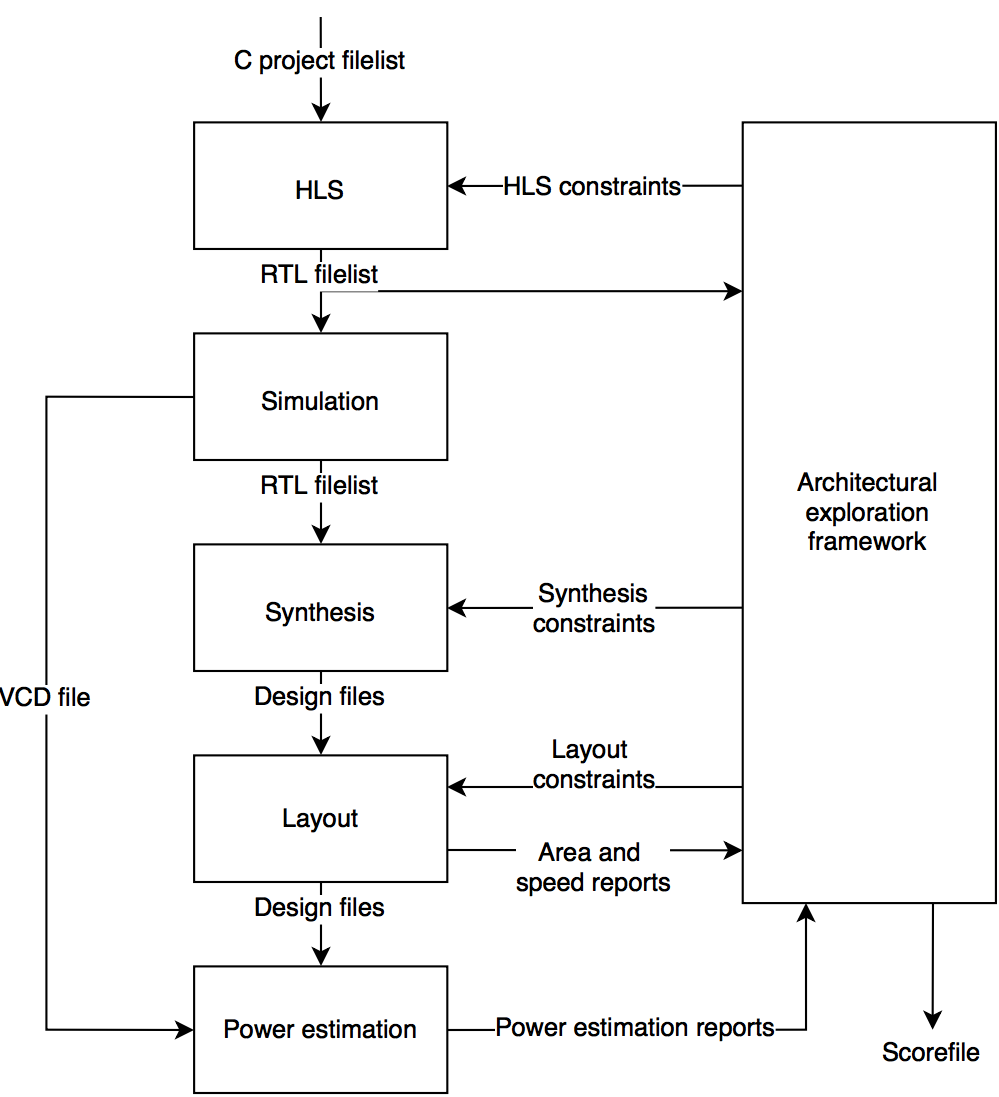
\includegraphics[width=0.6\textwidth]{../figs/Toolflow.png}
\caption{\label{fig:toolflowblock}Block diagram of tool-flow}
\end{figure}
Starting on the right side, a framework is created to control the flow, give constraints to the different steps and keep score of results. On the top of the figure, a filelist pointing to one or multiple C source files is input to the \gls{hls}-tool, in this case, LegUp. Based on the \gls{hls}-constraints given by the framework, LegUp will perform \gls{hls} on the given source files and output a \gls{rtl} filelist pointing to the generated Verilog source files. In the next step, simulation is run on the generated \gls{rtl} to generate a \gls{vcd} file needed for power estimation. It also makes sense to perform simulation in order to verify that the generated design functions properly and as expected. Synthesis and layout are then performed on the \gls{rtl} with respect to constraints given by the framework, generating area and speed reports, as well as post-layout netlist-files describing the final circuitry. In the final step, post-layout netlist files and the \gls{vcd} file from simulation are used to estimate power consumption. The report from power estimation are stored in the framework, together with area and speed results, given constraints and \gls{rtl} filelist. The Framework will run the whole tool-flow multiple times with varying constraints in order to find the best solution. When the tool-flow has been run for all desirable variations, the results will be compared and output in a score-file. This allows the designer to compare different architectural variations and select the best suited solution based on speed, area, and power requirements.

\section{Reference-design implementation}
In order to compare results of \gls{hls} generated code towards hand-written Verilog, the same reference design are created in both Verilog and C. The source code of each design are listed in \cref{sec:sourcecode}. Due to problems discussed in \cref{sec:encprob}, the designs have not been synthesised. It has therefore not been spent an extensive amount of time on verifying the correctness of the designs.
\subsection{FIR-filter}

The subsections below shows the algorithms and pseudocode for implementation of the reference desings.

\subsubsection{Verilog implementation}

A simple implementation of a FIR-filter is listed in \cref{lst:firfilterverilog}. The filter is converted to Verilog from a SystemVerilog example given in \cite{mehler2014digital}. This example is a direct form \gls{fir}-filter of N-order with a data pipeline of N-1. The filter operates on input data, and the output is full precision of internal caluclation. Parameters are included in the implementation to easily be able to change the width of the input or the depth of the pipeline.

\lstset{language=SystemVerilog, style=Verilogstyle}
\begin{lstlisting}[caption={FIR-filter implemented in Verilog},label=lst:firfilterverilog]
module direct2 #(WIDTH = 4, DEPTH = 4)
  (
	input ck, 
	input signed [WIDTH-1:0] dataIn,
	output logic signed[2*WIDTH-1+\$clog2(DEPTH):0] dataOut
	);
	
	logic signed [WIDTH-1:0] sr [DEPTH-2:0];
	logic signed [2*WIDTH-1:0] products [DEPTH-1:0];
	parameter logic signed [WIDTH-1:0] coeff [DEPTH-1:0] = {1,2,3,4};
	logic signed [2*WIDTH-1 + \$clog2(DEPTH):0] sum;
	// Test
	always_ff @(posedge ck) begin
		sr[0] <= dataIn;
		sr[DEPTH-2:1] <= sr[DEPTH-3:0]:
	end
	
	always_comb begin
		products[0] = dataIn * coeff[0];
		for (int i = 1; i < DEPTH; i++)
			products[i] = sr[i-1] * coeff[i];
	end
	
	always_comb begin
		sum = products[0]
		for (int i = 1; i < DEPTH; i++)
			sum = sum + products[i];
	end
	
	always_comb dataOut = sum;
endmodule
\end{lstlisting}
\subsubsection{C implementation}
The C implementation of the filter is also based on the SystemVerilog example from \cite{mehler2014digital}, to make the implementations comparable.
\lstset{language=C,style=Cstyle}
\begin{lstlisting}[caption={FIR-filter implemented in C},label=lst:firfilterc]

\end{lstlisting}


\subsection{SAP-1 Architecture}

\subsubsection{Verilog implementation}
The \gls{sap-1} architecture are easily implemented in Verilog. 
\subsubsection{C implementation}
When starting to design the \gls{sap-1} architecture in C, some potential problems were quickly discovered. The first problem is that it is hard to divide the architecture into the modules shown in \cref{fig:sap1arch}. The second problem is that it's hard to force the running of the program into 6 states, each lasting one clock cycle, when you have no control over the clock. When synthesizing the design into Verilog, it might be reduced to a single \gls{fsm}, doing all the work in just one cycle. The third problem is that as there are no bus capabilities in C, the data are just transferred using standard variables.


%%\chapter{Results and discussions}
\label{chp:resdisc}

\section{HLS output from LegUp}
As a quick introduction to how the output from LegUp looks, we will have a look at a simple example and what the output looks like. Since the code output is very large, it will be of more use to look at a figure describing the different parts of the code and how it is connected. Beware that this section describes output from LegUp when it is freshly installed, without any alterations or changes so setting. In general, the modules declared in the output Verilog file are these:
\begin{compactdesc}
    \item[top]Top module for Verilog. Instantiates main and memory\_controller modules.
    \item[main]Main function from C project. Contains \gls{fsm} that handles all functionality from original C program.
    \item[memory\_controller]Contains global memories and logic for reading and writing to memory. Instantiates as many ram\_dual\_port and rom\_dual\_port modules as necessary.
    \item[ram\_dual\_port] Dual port RAM module used inside memory controller for global memories.
    \item[rom\_dual\_port] Dual port ROM module used inside memory controller for global memories.
    \item[\%board\%]FPGA specific top module. Instantiates top-module and 8 hex{\textunderscore}digits modules and connects return\_value from top to hex modules for visualizing the results.
    \item[circuit\_start\_control]FPGA specific module. 
    \item[hex\_digits]FPGA specific module. Controls hex LEDs for visualization of results.
    \item[main\_tb]Basic testbench that can be used for simulation. Instantiates top-module. Testbench code generates \textit{clk} signal and applies \textit{reset} and \textit{start} signals to the module before waiting for finish flag. There are no additional input stimuli, so this needs to be added manually by the user.
\end{compactdesc}

\noindent
Listing \ref{lst:exampleCProgram} shows a simple C implementation of a square-root approximation. The reason that the arguments to the main function are given in this way, is described in \cref{subsec:inoutprobs}. \gls{hls} is performed by running \verb!make!. The output Verilog file contains over 3000 lines of code and can therefore not be presented her, it would anyway not give much information.
\begin{lstlisting}[caption={Useless code},label=lst:exampleCProgram]
#define abs(a) ( ((a) < 0) ? -(a) : (a) )
#define max( a, b ) ( ((a) > (b)) ? (a) : (b) )
#define min( a, b ) ( ((a) < (b)) ? (a) : (b) )

// square-root approximation:
int main(int inDataA, char *inDataB[]) {

    int x = max(abs(inDataA), abs(*inDataB[0]));
    int y = min(abs(inDataA), abs(*inDataB[0]));

    return max(x, x-(x>>3)+(y>>1));
}
\end{lstlisting}
\noindent
A project in Quartus can be created by running \verb!make p! and a full compilation can be executed by running \verb!make f!. The top module netlist of the example from \cref{lst:exampleCProgram} can be seen in \cref{fig:legupouttop}
\begin{figure}[hbpt]
\centering
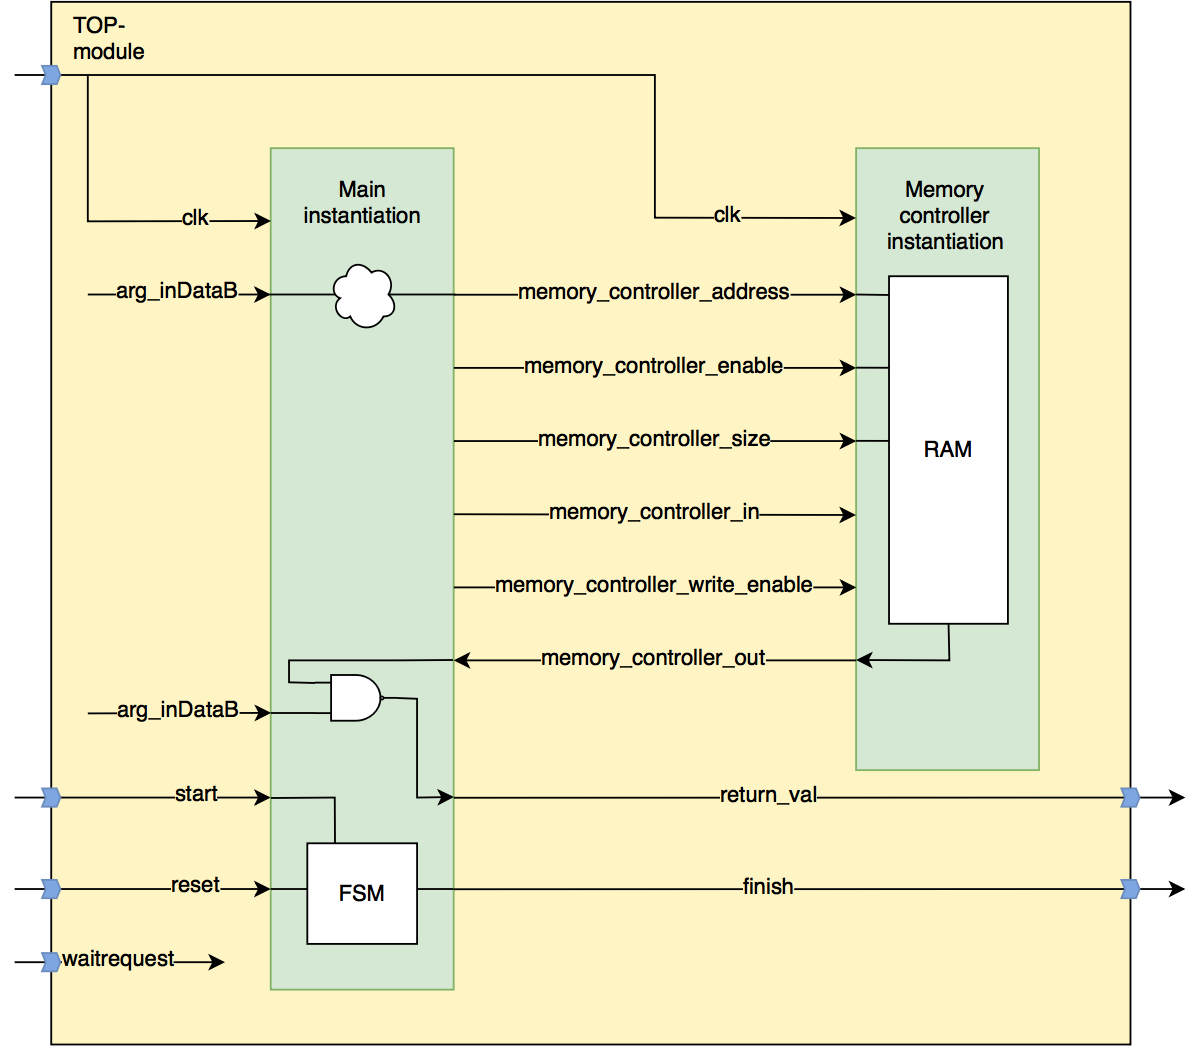
\includegraphics[width=\textwidth]{../figs/LegUpOutputTop.png}
\caption{\label{fig:legupouttop}Top module output from LegUp HLS}
\end{figure}
Notice that the inputs to the instantiated main module, inDataA and inData,B does not propagate to the top module instantiation. Also, if we look inside the main module, inDataB is only mapped to the signal \textit{memory\_controller\_address\_a}. This is because inDataB is decleared as a pointer in the C code, meaning that the input only provides the address to a location in memory where the data can be fetched. This issue is discussed further in \cref{sec:encprob}.

\begin{figure}[hbpt]
\centering
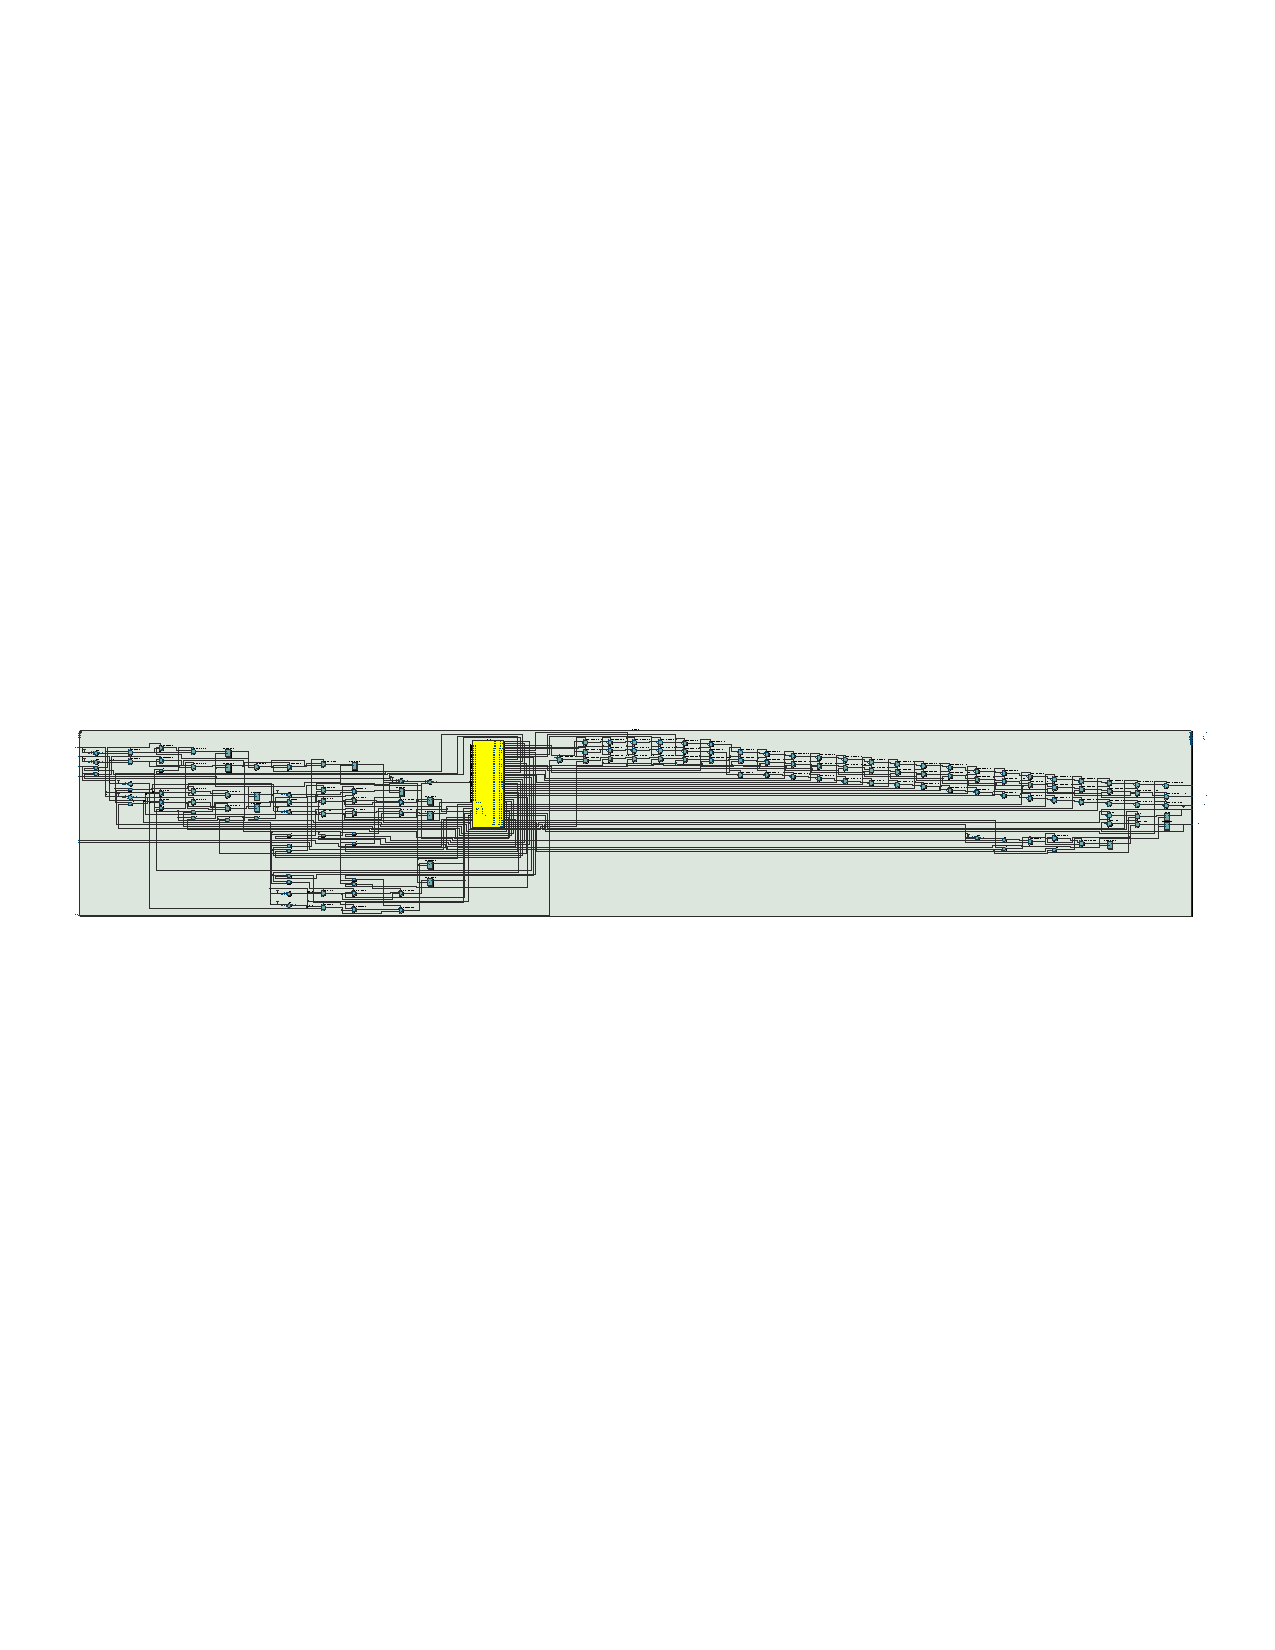
\includegraphics[width=\textwidth]{../figs/LegUpOutputMain.pdf}
\caption{\label{fig:legupoumain}Main module output from LegUp HLS}
\end{figure}

\section{\label{sec:encprob}Encountered problems}
Throughout the work with LegUp, multiple problems that limits its usefulness towards \gls{asic}-applications has been encountered. The following section will describe some of the problems and their implication for the synthesis results described in section \ref{sec:synthres}, as well as for the continuation of the project.
\subsection{\label{subsec:memctrl}Memory controller}
In order to communicate between different modules instantiated in the top-module of the output Verilog from LegUp, a memory controller is declared and instantiated. All variables detected as global by LegUp, i.e. variables used by multiple modules or declared as a pointer and the points-to analysis fails to determine the exact array for the pointer at compile-time, is stored in a \gls{ram} module inside this memory controller. This approach is well intended for the hybrid flow supported by LegUp, where a soft-processor works in cooperation with one or more functions implemented as hardware accelerators in an \gls{fpga}, meaning that data needs to be transferred between the software and hardware portion of the system. For an \gls{asic}, pure-\gls{hw} implementation however, this approach creates a lot of extra overhead and basically does not provide any additional functionality to the circuitry. In the pure-\gls{hw} flow in LegUp, all the functionality described under the main-function in the input C-code will be translated into a single \gls{fsm}. The main function is further the only module instantiated in the top-module of the produced Verilog, besides the memory controller. The use of the memory controller is in itself not an issue as LegUp handles all memory access automatically, but this will come at the expense of both decreased speed and increased area usage. It will also cause some problems related to input and output, as described in subsection \ref{subsec:inoutprobs}.
\subsection{\label{subsec:inoutprobs}Inputs and outputs}
When designing a hardware module, its task can vary almost infinitely. However, most modules take some data input together with some control signals, does something with the data and outputs some kind of response. This makes input and outputs, and the ability to configure them properly, extremely important in most module design. In the documentation of LegUp \cite{leguparch}, the developers claim that each function declared in C is translated into a corresponding module in Verilog. However, \gls{hls}-output shows that in the pure-\gls{hw} flow, the only generated module is the one containing the main-function, as describe in subsection \ref{subsec:memctrl}. As LegUp uses a standard C compiler front-end for \gls{llvm} to compile the C-code into \gls{llvm}-\gls{ir}, we need to follow the \gls{ansi}-C specification \cite{isoc} when writing our C-code. In a standard programming case, the \textit{main}-function has a special purpose, specifically, the run-time environment calls this function to start execution of the program. The return value of the main function is defined to be an int, who's purpose is to return program execution status to the invoker process. The main function is also defined to handle arguments input from command-line, through the input arguments \textit{int argc} and \textit{char *argv[]}, where \textit{argc} is the number of command-line arguments, and \textit{*argv} is an array of pointers to the given arguments. The implications of this is that if we want inputs and outputs to or from the module we design in out C-code, we are limited to the arguments allowed through the defined main-function in the \gls{ansi}-C specifications. Further, this problem increases when we realize that any inputs or outputs except one int for each has to be a pointer, which entails it has to go through the above described memory controller. This causes a lot of overhead, as most input- and output-data has to be written to and read from memory, creating the need for a dedicated custom module for handling I/O. A final issue related to input signals is that the given arguments to the main function in C are not propagated from the generated main module to the top module to make them inputs to the circuit. This means that the designer has to manually alter the generated Verilog to make the the arguments input signals, making it more difficult to create the desired automated framework.
\subsection{Bus widths}
When designing digital hardware circuits, you often want (and in some cases need) to use bit-vectors of a given size. \gls{ansi}-C does not have built-in support for data-types of other sizes than 8, 16, 32 and 64 bits, this cause problems when doing \gls{hls}. LegUp does however have a class, \textit{MinimizeBitwidth.cpp}, which calculate the minimum needed bits in a signal and limits the width to this size, but this does only work for internal signals, where all values assigned to the variable is known at compile-time. If the signal shall be an input or output, the maximum value of the signal is not known, and it can therefore not be limited. Having too wide signals will increase the occupied area as all components must support the extra bits. A simple example is shown in figure \ref{fig:andgate34}, where we can easily see that the addition of one extra bit to the input signal adds one extra 2-input AND gate to the circuit.
\begin{figure}[hbpt]
\centering
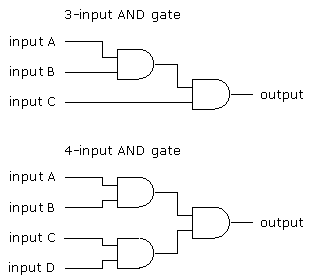
\includegraphics[width=0.6\textwidth]{../figs/AndGate34Bit.png}
\caption{\label{fig:andgate34}3-bit input versus 4-bit input AND-gate}
\end{figure}
Technically this is a limitation inherited from the lack of logical data-types in C, but this problem needs to be addressed if LegUp shall be used as an architectural exploration framework.
\subsection{\label{subsec:parameterprobs}Parameters}
The lack of support for transferring parameters from the C code into the generated Verilog makes it harder to instantiate modules based on widths or depths of different parameters. Often this is desirable in order to reuse the modules for a variety of given parameter values.
\section{\label{sec:synthres}Synthesis results}
Due to the above mentioned problems, some manual alteration of the generated Verilog had to be made in order for the results from LegUp to be comparable to the results from the native Verilog.

\section{Tool-flow and script}
Due to that the \gls{hls}-tool, LegUp, is located on a VirtualBox image while the synthesis and power-estimation tools are located on Nordic's servers, it is not possible to make a single workflow.
%%\chapter{Discussion}
\label{chp:discussion} 
%%\chapter{Conclusion}
\label{chp:conclusion} 
%% include here the other chapters

\renewcommand*{\bibname}{References}
\bibliographystyle{plain}
\bibliography{main}

%% Uncomment the following if you have any appendix
% \appendix
% \addtocontents{toc}{%
%  \protect\vspace{1em}% 
%  \protect\noindent \bfseries \appendixtocname\protect\par
%  \protect\vspace{-.5em}%
% }
% \renewcommand{\chaptername}{\appendixname}
%% include below possible appendices (chapters)


\end{document} 
